\documentclass[a4paper]{article}
\usepackage[english]{babel}
\usepackage[utf8x]{inputenc}
% package for including graphics with figure-environment
\usepackage{graphicx}
\usepackage{hyperref}
\usepackage{multirow}
\usepackage[official]{eurosym}
\usepackage[final]{pdfpages}
\usepackage{listings}

\usepackage{pgfplots}
\pgfplotsset{width=10cm,compat=1.9}
%\usepgfplotslibrary{external}
%\tikzexternalize


% colors for hyperlinks
% colored borders (false) colored text (true)
\hypersetup{colorlinks=true,citecolor=black,filecolor=black,linkcolor=black,urlcolor=black}

\lstset{frame=tb,
  language=Java,
  breaklines=true,
  showstringspaces=false,
  columns=flexible,
  numbers=none,
  commentstyle=\color{dkgreen},
  stringstyle=\color{mauve},
  tabsize=3
}

% package for bibliography
\usepackage[authoryear,round]{natbib}
% package for header
\usepackage[automark]{scrpage2}
\pagestyle{scrheadings} 
\ohead[]{\today}
\cfoot[]{\pagemark} 
\setheadsepline[122mm]{0.3mm}
\begin{document}
	\title{
	\begin{figure}[!ht]
		% \flushleft
			
\includegraphics[width=0.26\textwidth]{THlogoheader.pdf}
	\end{figure}
	\vspace{1cm}
	\Huge Web Architecture private Portfolio
	}
	
	\vspace{1cm}
	
	% if you are the only author, you might use the following
	% \author{Name of student}	
	% Insert here your name and correct mail address
	\author{\Large \href{}{Franziska Schmidt} \and \Large  \href{}{Kyung Hee Lee} \and \Large  \href{mailto:krzysztof_jedrzej.dabrowski@smail.th-koeln.de}{Krzysztof Dabrowski} \and \Large  
	\vspace{1cm}}
	
	% name of the course and module
	\date{
	\large Module: Fundamentals I \\ Course: Visualisation \\ 
	\vspace{0.8cm}
	\large Lecturer: Prof. Dr. Martin Eisemann \\
	\vspace{1cm}
	\today
	}

	\maketitle
	\setlength{\parindent}{0pt}

\vspace{2cm} 
	\newpage
	
\section{Motivation and Background of the visualisation} % (fold)
The motivation of this project is the current discussion about global warming. Currently we develop an app to improve the environmental behavior of people. It is important in order to change something to know the reasons for the climate change. One reason is the co2 pollution. To understand the co2 pollution one has to consider the emerge during the years. Furthermore the distribution of co2 emission in the world will give interesting insights about the activities of the individual countries.


\section{Related Work}
\section{Project Objectives and Goals}
\section{Data}
\section{Data Processing}
Data Model: Low-level description of the data 
Set with operations, e.g., floats with +, -, /, * 
Conceptual Model: Mental construction 
Includes semantics, supports reasoning 
Visual Variable: Visual Representation 
Mapping of data to a coherent visual representation


Quantitative: Can we quantify the difference between two marks


\section{Visualisation Design}

The visual design was developed by considering Edward
R. Tufte's heuristics and principles.
"Graphical excellent is that which gives to the
viewer the greatest number of ideas in the shortest time with the least ink in the
smallest space."\cite{Tufte2001} The least ink ratio hints to one of Tufte's heuristics, which is "maximize the data Ink ratio. \\
\\ $\frac{data-ink}{total ink used to print the graphic (data-ink + non data-ink)}$ \\
\newline The relationship between the data ink which is the ink used for the data itself (key informations) and the total amount of ink of the whole visualisation form the data ink ratio.
That means that visualisations should be as simple as possible while showing all relevant information.
The other heuristics are:
\begin{itemize}
    \item Avoid chart junk 
\item Increase data-density 
\item Layering of information
\end{itemize}{}
Our visualization is divided into two parts. The first part is the CO2 - Emission of one or more countries over the years (see Figure 1). 

\begin{figure}[h!]
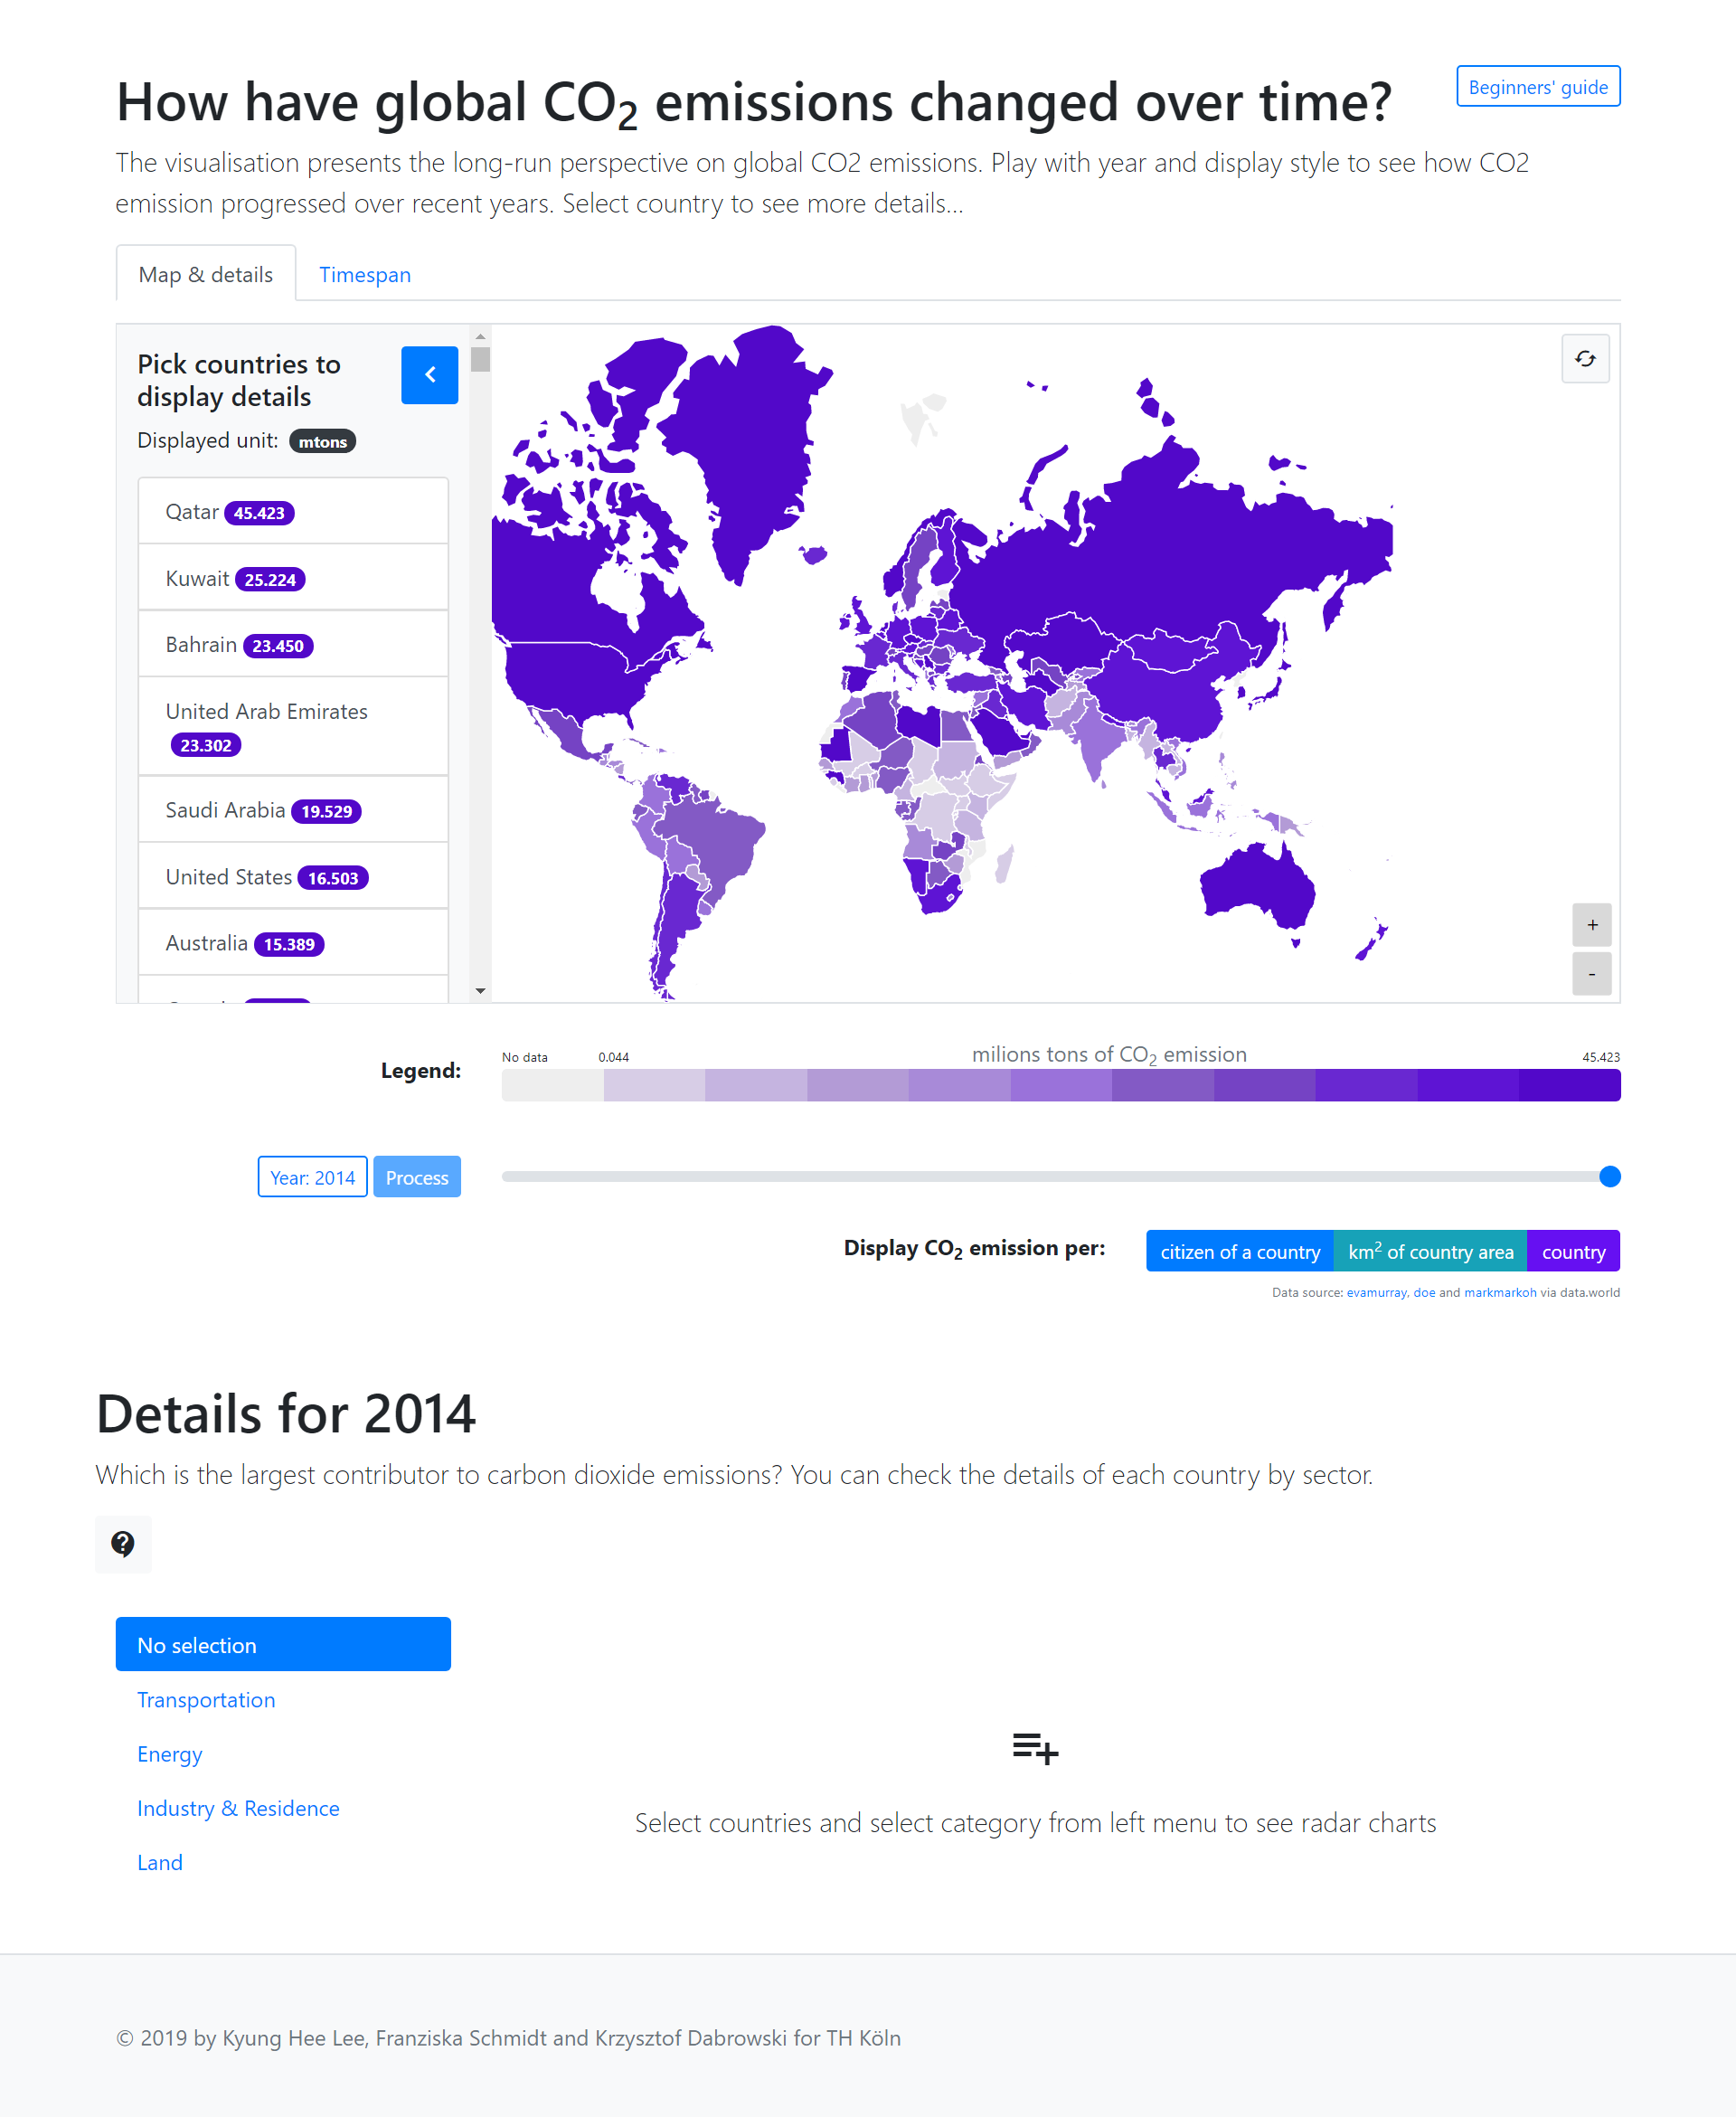
\includegraphics[width=1.0 \textwidth]{screencapture-glanonim-Archive-visualization-2020-01-12-17_46_35.png} 
\caption{Screenshot of the First state of the visualisation}
\end{figure}
\subsection{Map and Details Tap} 
Firstly the information is displayed on a map. Colour is used to show the CO2 emission of a country in millions of tons. The colour span is going from grey to different shades of purple. 
\\ The darker the purple the higher the amount of co2 is. The colour purple was chosen because there shouldn't be a judgement implicated by the chosen colour. Furthermore the implementation tool only allows two colours. \\

\\ "To avoid chart junk" the interactive elements are shared with the different visualization. When they are once chosen by the user they are valid for all of the visualizations. They are placed next to the central visualization (the map), because it is the first thing a user should do. The map has two serving purposes for the whole visualization. First of all it gives an overview about the co2 emissions of the country. Secondly it is an interactive element for the user to select the countries he would like to know more about. This encourages the experimentation and exploration, because it is more playful than selecting the countries in a list. The map is also visually more attractive than a list. Nevertheless, a list of countries is placed on the left hand side of the map. This supports the users in finding and selecting a specific country they are looking for. For some user it might also be hard to select small countries on a map. Although a zooming function is available.
\\ Shneiderman Mantra „Overview first, zoom and filter, then details-on-demand“ helped to find the design solution. The map gives the overview and the zoom supports the user later. The "details on demand" is there as well, because the countries react on hovering over the countries. Additional information are displayed then like the countries name. The colour purple represents "co2 emission per country". The Map also offers "co2 emission per km2 of a country area" and "co2 emission per citizen of a country". This options can be chosen in a legend beneath the map on the right hand side. When changing to another option the whole map and reference information change to the colour blue or turquoise. The colour options all belong to the blue colour group. Blue is associated also with air. Which matches the content but is at the same time also not implicating a judging. 
Another interaction with the map is a timeline year selector. The user can select the year he wants to look at the data. Furthermore he can click on a play-button to see a automated timeselection. 
 He sees the evolution of co2 of the different countries over the different years. \\ 
With the Interaction Tufte’s Integrity Principles:
"Show data variation, not design variation" and  
"Clear, detailed, and thorough labeling should be used to defeat graphical distortion and ambiguity" \cite{Tufte2001} are followed. The different variations who can be chosen by the user are data variations and not design variations. 
\\
\subsubsection{Details}
Beneath the Map Area there is the "Details" - part. When a user selected more than one country he can press on the "process"- Button. The "Details" are about the categories: Transportation, Energy, Industry and Residence and Land. The further information is about the selected year and helps the user to compare different countries. 
\newpage

\begin{figure}[h!]
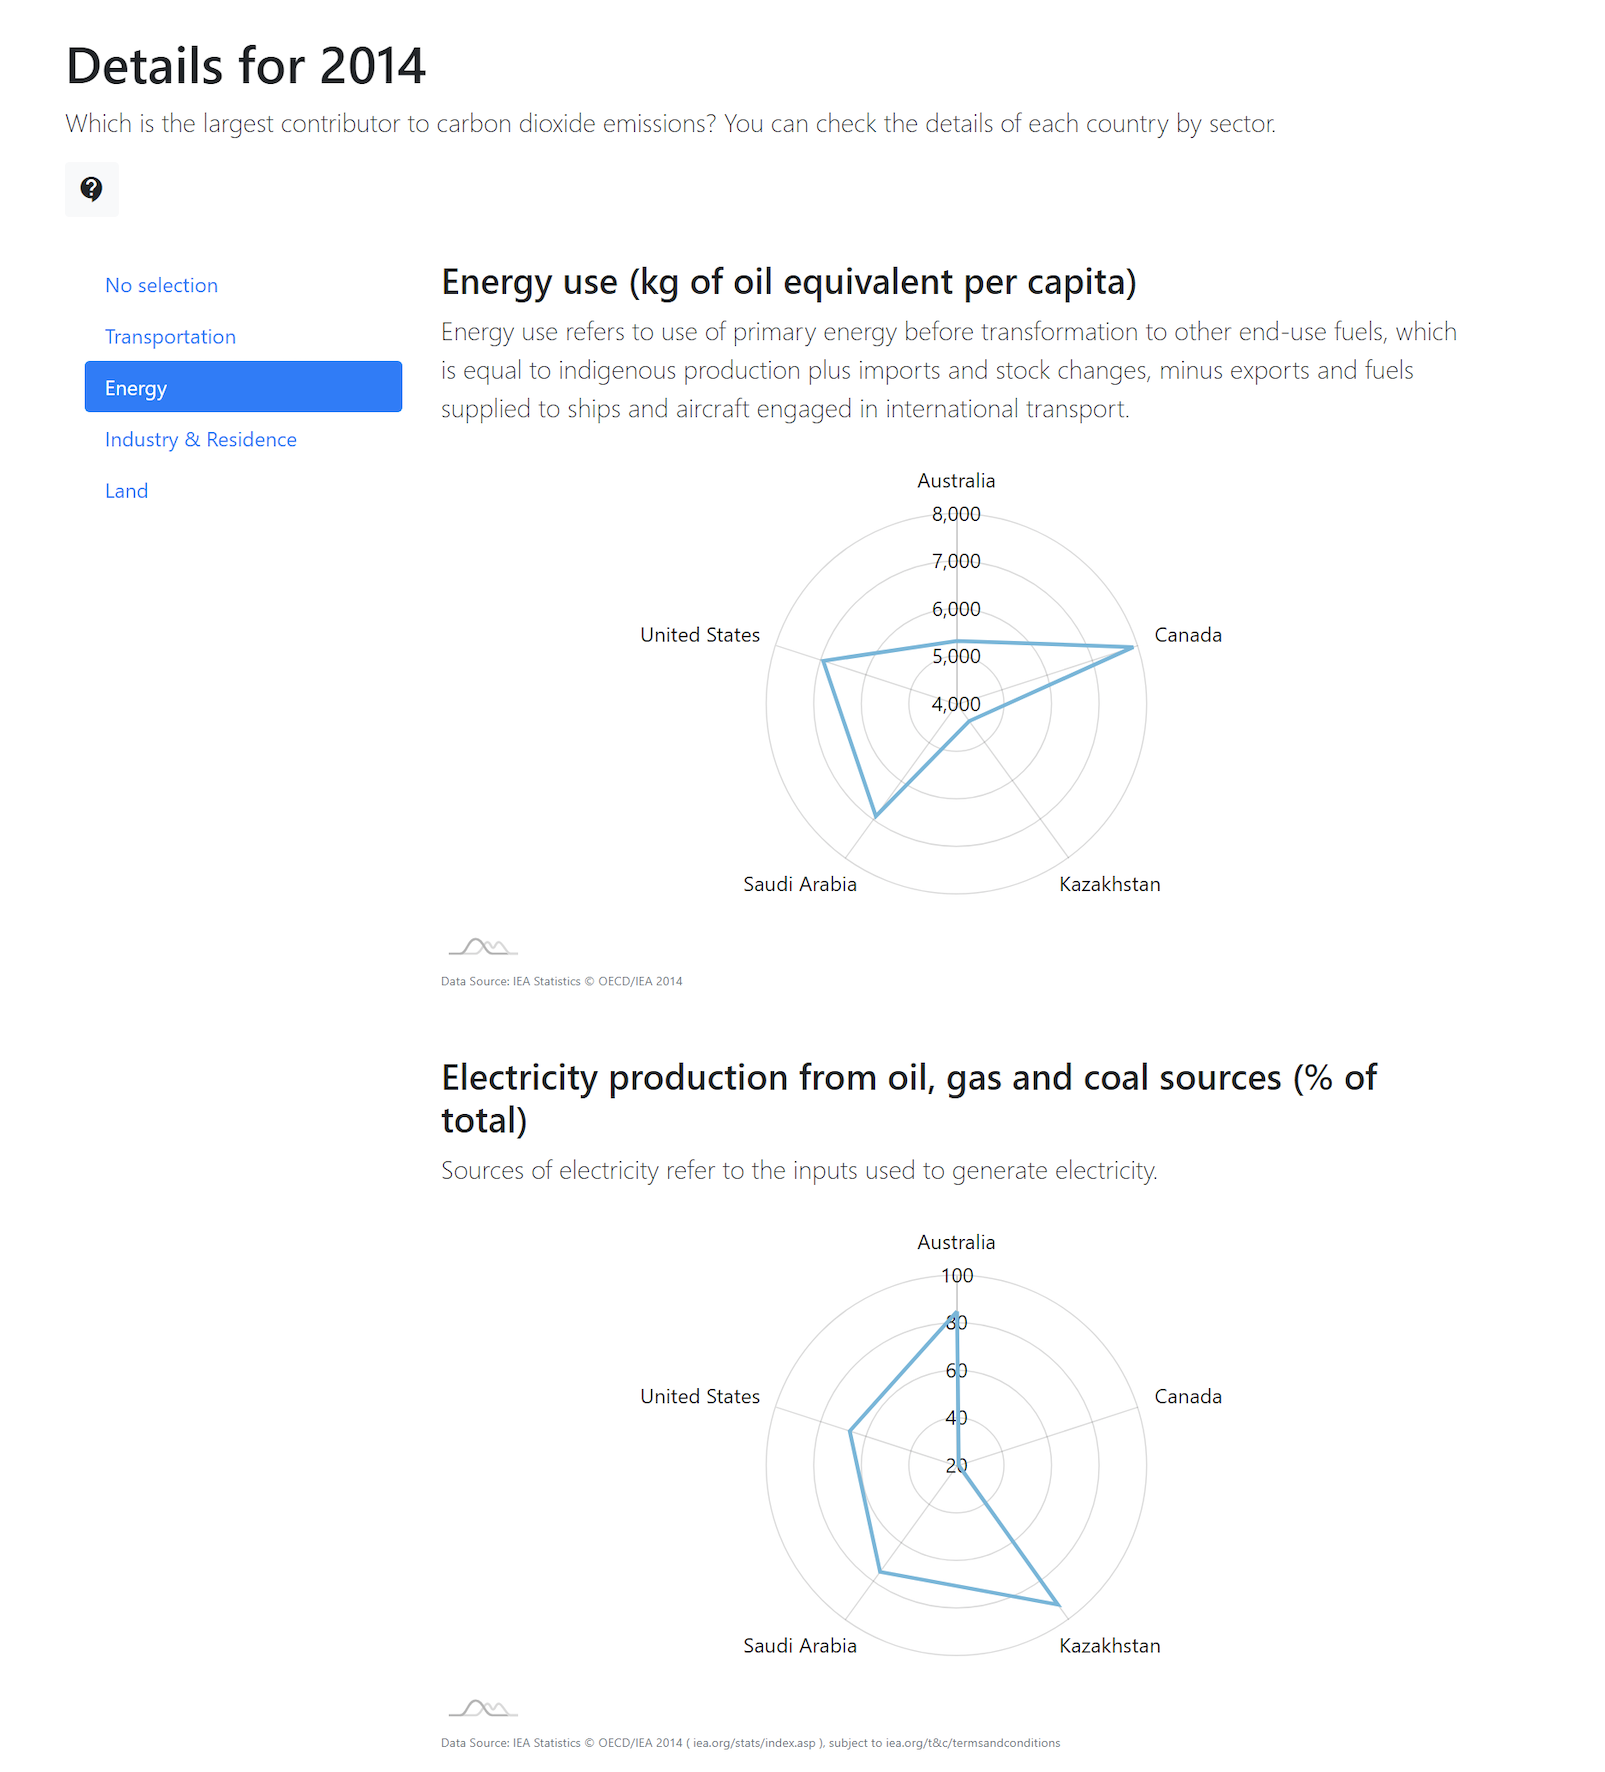
\includegraphics[width=1.0\textwidth]{detail.png} 
\caption{Screenshot of the Details part}
\end{figure}

Figure 2 shows the Details for 2014 on the Tap Energy. The title and a short description of the used data helps the user to understand the chart and displayed data. We decide to display the data in a radar chart, because it helps comparing multiple quantitative variables. The gridlines help to see the value of the variable. The exact value is harder to see, but the intend of this graphic is to compare the different countries. The shape of the gridlines support the user in seeing similar values and whether there are any outliers amongst each variable. We decide due to Tufte's least ink rule not to fill the gab between the gridlines. Furthermore this would hide the scale. 
\newpage
\section{Timespan Tap}
\begin{figure}[h!]
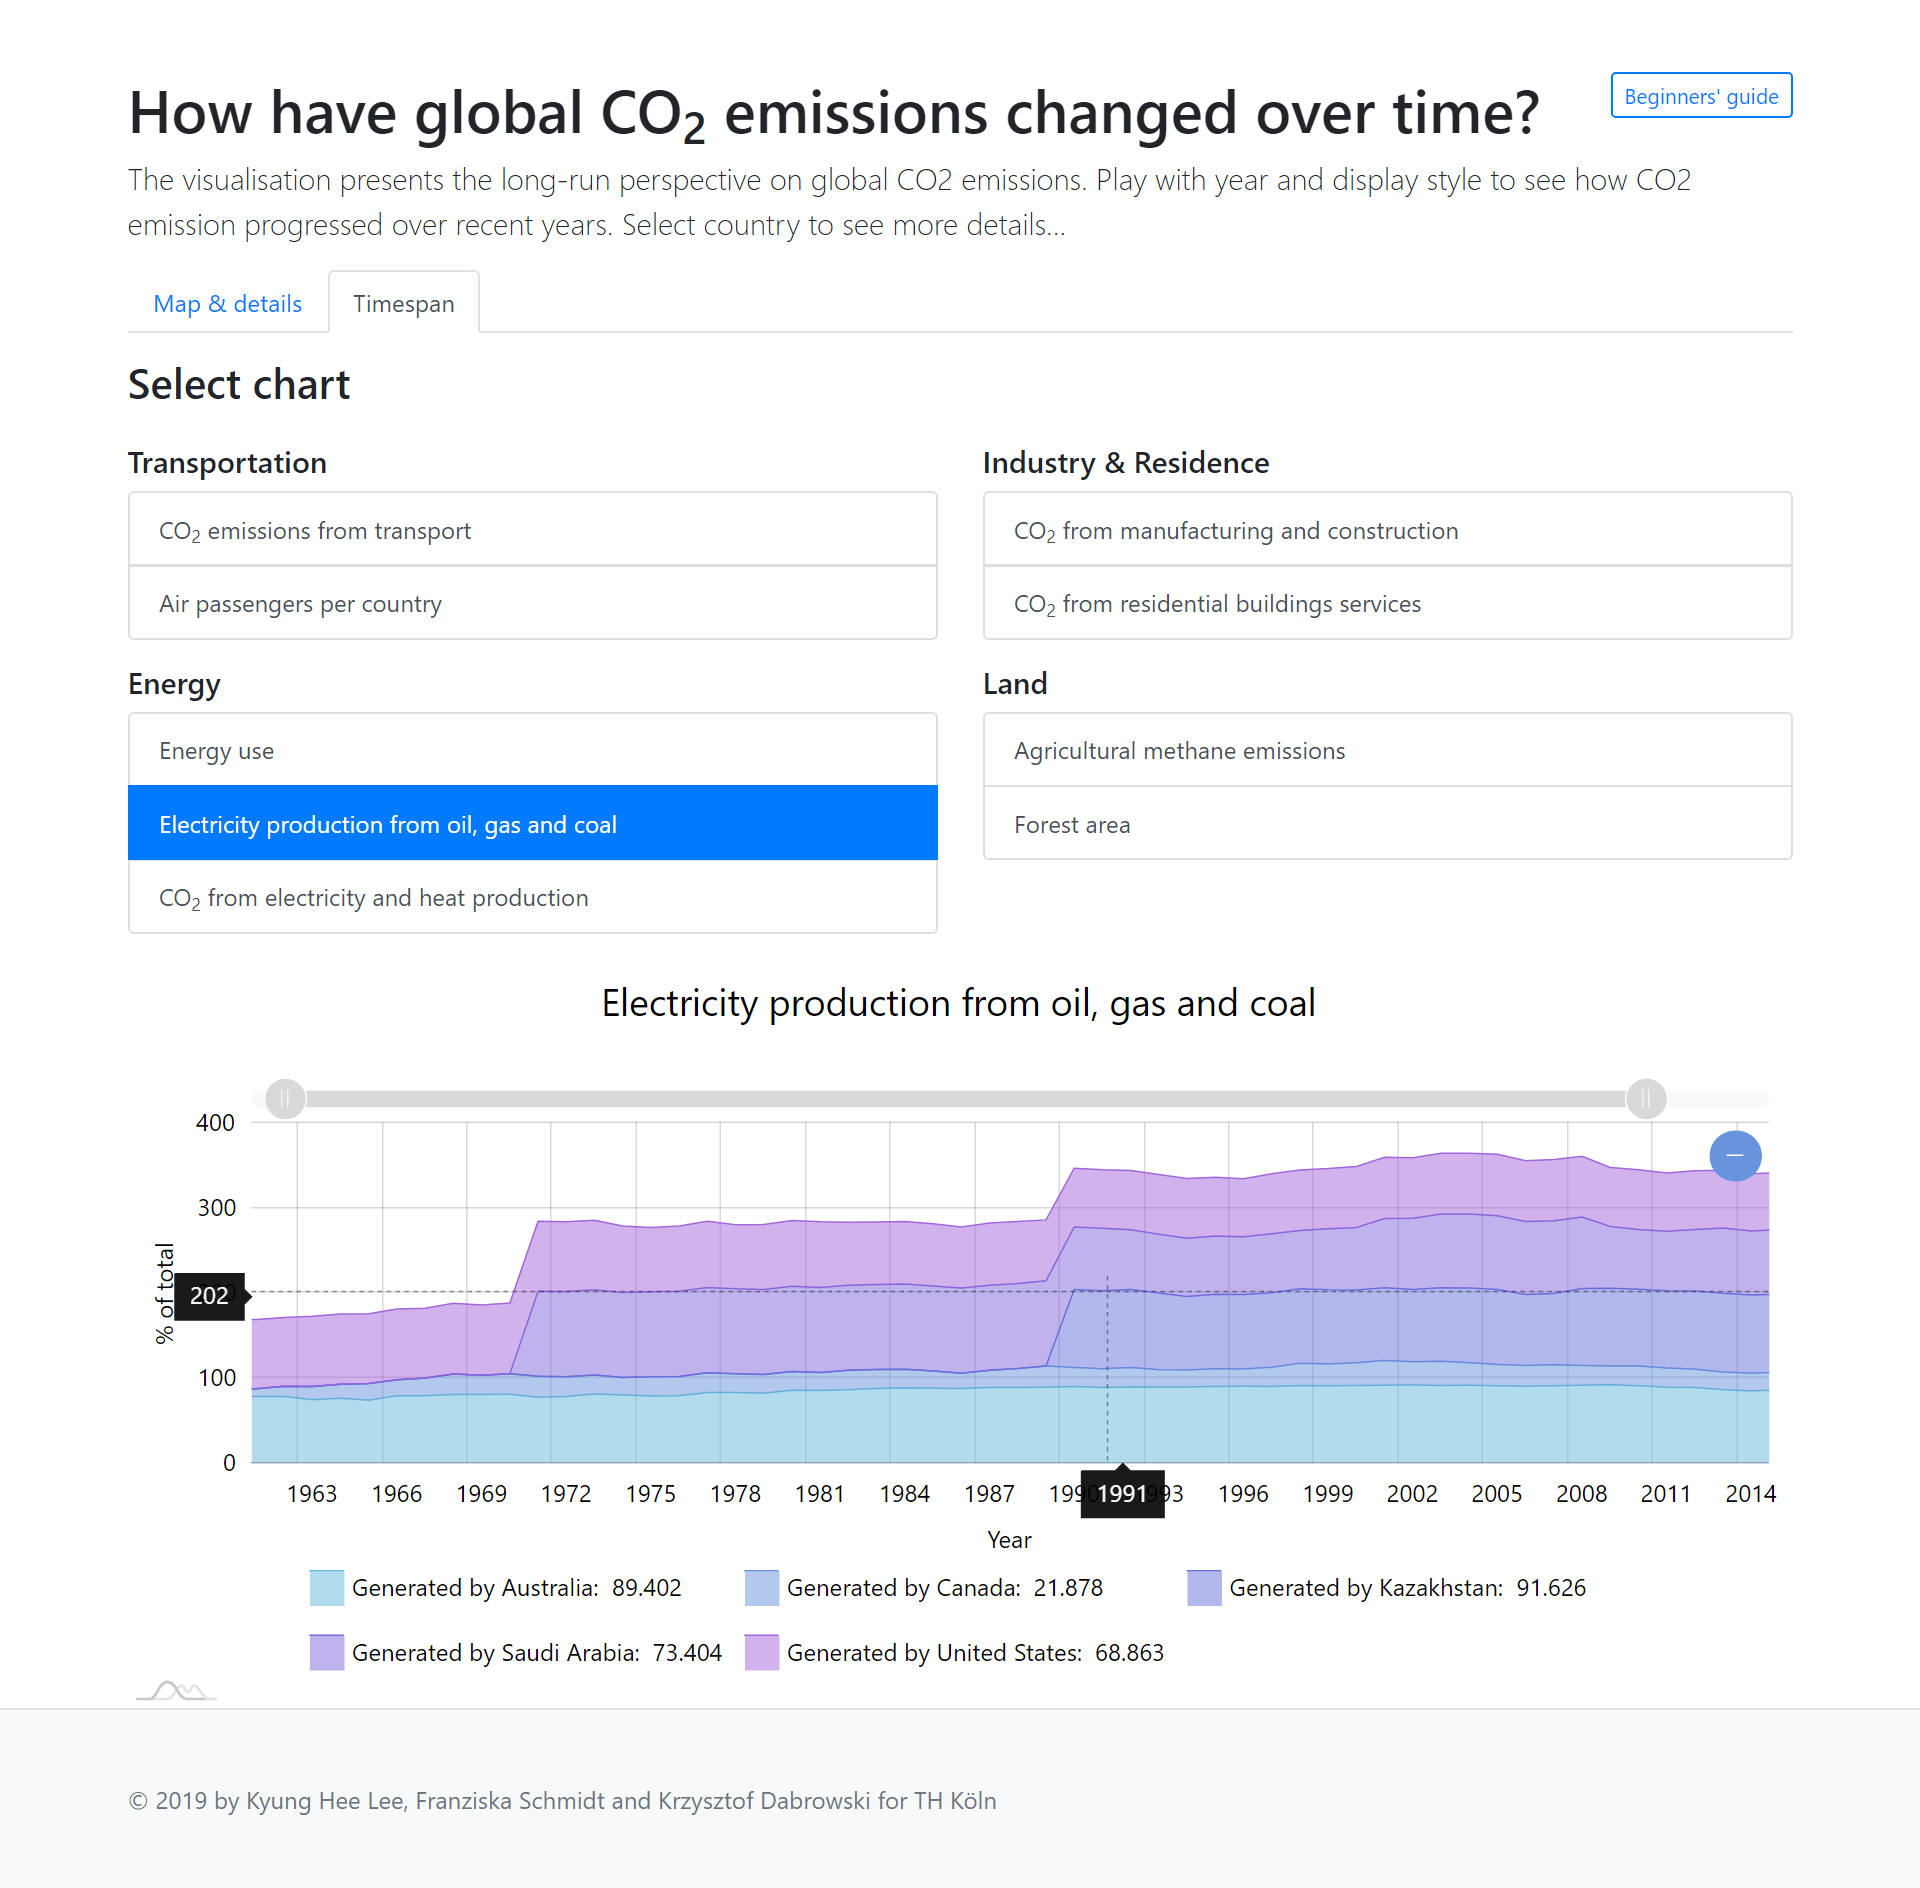
\includegraphics[width=1.0\textwidth]{screencapture-glanonim-Archive-visualization-2020-01-12-17_49_13.png} 
\caption{Screenshot of the Timespan Tap}
\end{figure}

\section{Tasks}
\section{Must-Have Features}
\section{Optional Features.}
\section{Project Schedule}
\section{Implementation details}

\end{document}